\documentclass[table]{beamer}

\usepackage{kotex}
\usepackage{amsmath}
\usepackage{amssymb}
\usepackage{verbatim}
\ifxetex
 \setsansfont{TeX Gyre Heros}
 \setsanshangulfont{맑은 고딕}
\fi
\usepackage{color, colortbl}					%tabular에서 rowcolor를 변경하기 위해서..
\usepackage{fancybox}
\usepackage{graphbox,graphicx}
\usepackage{tikz}								%오버레이에 그림을 그리기 위해서..
\usepackage{hyperref}							%하이퍼링크 처리

\usepackage{array}
\usepackage{ebproof}
\usepackage{multirow}


\usepackage{xcolor,multirow}
\usepackage{hhline}

\usepackage[T1]{fontenc}
\usepackage{textcomp}
\usepackage{listings}							%자바 코드를 위해서..
\lstset{
	mathescape,
	language=Java,
	basicstyle=\footnotesize\ttfamily,
	keywordstyle={}, % \footnotesize\color{blue}\ttfamily,
	captionpos=b,
	escapeinside=@@,
	showstringspaces=false,					%공백 문제 제거를 위해서
	tabsize=2,
	upquote=true
}

%----------------- 총 페이지수에서 백업 슬라이드를 제거하기 위해서....
\newcommand{\backupbegin}{
   \newcounter{framenumberappendix}
   \setcounter{framenumberappendix}{\value{framenumber}}
}
\newcommand{\backupend}{
   \addtocounter{framenumberappendix}{-\value{framenumber}}
   \addtocounter{framenumber}{\value{framenumberappendix}} 
}
%-----------------

%---------------- tabular에서 rowcolor를 변경하기 위해서..
\definecolor{Gray}{gray}{0.9}
%-----------------

%\usetheme{CambridgeUS}
% \usecolortheme{default}

\usetheme{default}
\usecolortheme{default}

%\usetheme{default}
%\usecolortheme{beaver}
%\usetheme{CambridgeUS}
%\usecolortheme{seagull}

%\useinnertheme{rectangles}


\setbeamertemplate{caption}{\insertcaption}	%그림의 캡션 자동 만들지 않도록.

\addtobeamertemplate{navigation symbols}{}{%
    \usebeamerfont{footline}%
    \usebeamercolor[fg]{footline}%
    \hspace{1em}%
    \insertframenumber/\inserttotalframenumber
}

\title[Types and Programming Languages]{5. The Untyped Lambda-Calculus \\
(Types and Programming Languages)}
\author[K. Choi]{Kwanghoon Choi}
\institute[Chonnam National University]{
Software Languages and Systems Laboratory \\
	Chonnam National University}
\date{Week 5}

%%%%% Macros %%%%%

\newcommand{\rpc}{$\lambda_{rpc}$}
\newcommand{\polyrpc}{$\lambda_{rpc}^{\forall}$}
\newcommand{\stateencrpc}{$\lambda_{rpc}^{enc}$}
\newcommand{\statefulrpc}{$\lambda_{rpc}^{state}$}

\newcommand{\cs}{$\lambda_{cs}$}
\newcommand{\stateenccs}{$\lambda_{cs}^{enc}$}
\newcommand{\statefulcs}{$\lambda_{cs}^{state}$}

\newcommand{\client}{\textbf{c}}
\newcommand{\server}{\textbf{s}}
\newcommand{\clientserver}{\textbf{cs}}

\newcommand{\Loc}{Loc}

\newcommand{\evalRPC}[3]{#1\Downarrow_{#2}#3}
\newcommand{\evalRPCC}[2]{#1\Downarrow_{\client}#2}
\newcommand{\evalRPCS}[2]{#1\Downarrow_{\server}#2}
\newcommand{\lamL}[3]{\lambda^{#1}#2.#3}
\newcommand{\appL}[3]{#1{\ }^{#2}#3} 
\newcommand{\subst}[2]{\{#1/#2\}}
\newcommand{\llet}[3]{\textsf{let} \ #1 = #2 \ \textsf{in} \ #3}

\newcommand{\textsfReq}{\textsf{req}}
\newcommand{\req}[2]{\textsfReq(#1,#2)}
\newcommand{\reqwith}[3]{\textsfReq_{#1}(#2,#3)}

\newcommand{\textsfCall}{\textsf{call}}
\newcommand{\call}[2]{\textsfCall(#1,#2)}
\newcommand{\callwith}[3]{\textsfCall_{#1}(#2,#3)}

\newcommand{\textsfRet}{\textsf{ret}}
\newcommand{\ret}[1]{\textsfRet(#1)}
\newcommand{\retwith}[2]{\textsfRet_{#1}(#2)}

\newcommand{\funL}[1]{\xrightarrow{#1}}    
\newcommand{\funLC}[2]{\xrightarrow[#2]{#1}}  
\newcommand{\tyenv}{\Gamma}     
\newcommand{\tyenvExt}[2]{\Gamma\{#1:#2\}}
\newcommand{\tyenvExtWith}[1]{\Gamma,#1}
% \newcommand{\typing}[4]{#1\rhd_{#2} #3 : #4}       
\newcommand{\typing}[4]{#1\vdash_{#2} #3 : #4}       
\newcommand{\typingBlack}[4]{#1\blacktriangleright_{#2} #3 : #4}  

\newcommand{\loceta}[2]{{#1}\rightsquigarrow{#2}}                                         

\newcommand{\enc}{\textsf{enc}}
\newcommand{\evalStateEncRPCC}[2]{$#1\Downarrow_{\client}^{\enc}#2$}
\newcommand{\evalStateEncRPCS}[3]{$#1;#2\Downarrow_{\server}^{\enc}#3$}

\newcommand{\sta}{\textsf{state}}
\newcommand{\evalStatefulRPCC}[3]{\evalStatefulRPC{#1}{#2}{\client}{#3}}
\newcommand{\evalStatefulRPCS}[3]{\evalStatefulRPC{#1}{#2}{\server}{#3}}
\newcommand{\evalStatefulRPC}[4]{${#1};{#2}\Downarrow_{#3}^{\sta}{#4}$}

\newcommand{\deep}{\textsf{deep}}
\newcommand{\evalDeeplyStatefulRPCC}[3]{\evalDeeplyStatefulRPC{#1}{#2}{\client}{#3}}
\newcommand{\evalDeeplyStatefulRPCS}[3]{\evalDeeplyStatefulRPC{#1}{#2}{\server}{#3}}
\newcommand{\evalDeeplyStatefulRPC}[4]{${#1};{#2}\Downarrow_{#3}^{\deep}{#4}$}

\newcommand{\IdK}{\textsf{Id}}
\newcommand{\FunK}[3]{\textsf{Fun} \ #2 \ #3}
\newcommand{\AppK}[3]{\textsf{App} \ #2 \ #3}
%\newcommand{\FunK}[3]{\textsf{Fun}^{#1} \ #2 \ #3}
%\newcommand{\AppK}[3]{\textsf{App}^{#1} \ #2 \ #3}
                                                
\newcommand{\reify}[1]{\ulcorner #1 \urcorner}

\newcommand{\RightarrowEnc}{\Rightarrow^{enc}}
\newcommand{\RightarrowEncStar}{\Rightarrow^{enc*}}
\newcommand{\RightarrowEncPlus}{\Rightarrow^{enc+}}

\newcommand{\runStateEncRPC}[2]{$#1 \RightarrowEnc #2$}
\newcommand{\runStateEncRPCStar}[2]{$#1 \RightarrowEncStar #2$}
\newcommand{\runStateEncRPCPlus}[2]{$#1 \RightarrowEncPlus #2$}

\newcommand{\runStateEncCS}[2]{$#1 \Rightarrow^{enc} #2$}
\newcommand{\runStateEncCSStar}[2]{$#1 \Rightarrow^{enc*} #2$}

\newcommand{\runStatefulRPC}[2]{$#1 \Rightarrow^{state} #2$}
\newcommand{\runStatefulRPCStar}[2]{$#1 \Rightarrow^{state*} #2$}

\newcommand{\runStatefulCS}[2]{$#1 \Rightarrow^{state} #2$}
\newcommand{\runStatefulCSStar}[2]{$#1 \Rightarrow^{state*} #2$}

\newcommand{\emp}{\epsilon}
\newcommand{\substzsxs}{\{\bar{v}/\bar{z},\overline{w}/\bar{x} \}}
\newcommand{\substxs}{\{\overline{w}/\bar{x} \}}

\newcommand{\substZsXs}{\{\overline{V}/\bar{z},\overline{W}/\bar{x} \}}
\newcommand{\substXs}{\{\overline{W}/\bar{x} \}}

\newcommand{\LetK}[2]{\textsf{ctx}\ #1 \ #2}
%\newcommand{\LetK}[2]{(#1,#2)}
\newcommand{\opt}[1]{#1_{opt}}

\newcommand{\overlineK}{\overline{K}}
\newcommand{\overlinePi}{\overline{\Pi}}
\newcommand{\overlineDelta}{\overline{\Delta}}

%\newcommand{\comp}[1]{\rightsquigarrow_{#1}}
%\newcommand{\comps}{\rightsquigarrow_{\server}}
%\newcommand{\compc}{\rightsquigarrow_{\client}}
\newcommand{\ccomp}[1]{C[\![#1]\!]}
\newcommand{\scomp}[1]{S[\![#1]\!]}
\newcommand{\vcomp}[1]{V[\![#1]\!]}
\newcommand{\cconv}[1]{CC[\![#1]\!]}
%\newcommand{\cconvprg}[1]{CC_{prg}[\![#1]\!]}

\newcommand{\FUNS}{\Phi}
\newcommand{\fv}[1]{\textsf{fv}(#1)}
\newcommand{\dom}[1]{\textsf{dom}(#1)}
\newcommand{\clo}[2]{clo({#1},{#2})}

\newcommand{\sessionNothing}{\makebox[0.3cm][c]{\scriptsize $nothing$}}
\newcommand{\sessionSomething}{\makebox[0.3cm][c]{\scriptsize $session$}}
\newcommand{\sessionOption}{\makebox[0.3cm][c]{\scriptsize $optSession$}}

\newcommand{\mono}[1]{[\![#1]\!]}

\newcommand{\eqdef}{\overset{\mathrm{def}}{=\joinrel=}}

%%
%\newtheorem{lemma}{Lemma}[section]
%\newtheorem{theorem}{Theorem}[section]
%\newtheorem{fact}{Fact}[section]
%\newtheorem{definition}{Definition}[section]

%%%%%%%%%%%%%%%%%%

\begin{document}

%\section{Relative Pronoun}
\begin{frame}
%\begin{center}
%{\footnotesize
%Types and Programming Languages
%}
%\end{center}
	\titlepage
	
%	\begin{center}
%	{
%  (Joint work with James Cheney, Simon Fowler, and Sam Lindley)
%	}
%	\end{center}
\end{frame}

%\begin{frame}{Table of Contents}
%\begin{itemize}
%\item
%\item
%\item
%\item
%\end{itemize}
%\end{frame}

%%%
\begin{frame}[t]{Overview} \vspace{10pt}

This chapter introduces the {\it untyped or pure lambda calculus} (Alonzo Church 1936, 1941). 

\vspace{10pt}

Every complex programming language can be understood by formulating it as 
\begin{itemize}
\item \underline{a tiny core calculus} capturing the language's essential mechanisms, together with
\item \underline{a collection of convenient {\it derived forms}} whose behavior is understood by translating them into the core. 
\end{itemize}
(Peter Landin 1964, 1965, 1966; John McCarthy 1959, 1981)

\vspace{10pt}

The lambda calculus has seen widespread use in the design and implementation of PLs and in the study of type systems.

\vspace{10pt}

The core calculus in Ch.5, its type system in Ch.9, and the derived forms in Ch.11, Ch.13, Ch.14.

\end{frame}

%%%
\begin{frame}[t]{Overview (Cont.)} \vspace{10pt}

The lambda calculus can be enriched in a variety of ways.

\vspace{10pt}

First, it is often convenient to add special concrete syntax for features like numbers, tuples, records, etc., whose behavior can already be simulated in the core language (Ch.11). 

\vspace{10pt}

More interestingly, we can add more complex features such as mutable reference cells (Ch.13) or nonlocal exception handling (Ch.14), which can be modeled in the core language only by using rather heavy translations.

\vspace{10pt}

Such extensions lead eventually to languages such as ML, Haskell, or Scheme. 

\vspace{10pt}

The extensions to the core language often involve extensions to the type system as well.  

\end{frame}


%%%
\begin{frame}[t]{5.1 Basics} \vspace{10pt}

Procedural (or functional) abstraction: Instead of writing the same calculation over and over, we write a procedure or function that performs the calculation generically.

\vspace{10pt}

(5*4*3*2*1) + (7*6*5*4*3*2*1) - (3*2*1) \\
vs. 
factorial(5) + factorial(7) - factorial(3) \\
\ \ \ \ \ where factorial(n) = if n=0 then 1 else n*factorial(n-1)

\vspace{10pt}

Notation: \\
``$\lambda n. \ ...$'' as a shorthand for ``the function that, for each $n$, yields ...''

\vspace{10pt}

factorial = $\lambda n$. if n=0 then 1 else n*factorial(n-1)

\end{frame}

%%%
\begin{frame}[t]{5.1 Basics} \vspace{10pt}

The lambda-calculus (or $\lambda$-calculus) embodies this kind of function definition and application in the purest possible form. 

\vspace{10pt}

The syntax of the lambda calculus
\[
t \ ::= \ x \ \ \ | \ \ \ \lambda x. t \ \ \ | \ \ \ t \ t 
\]
where the three sorts of terms are called \underline{variable}, \underline{abstraction}, and \underline{application}, respectively.

\end{frame}

%%%
\begin{frame}[t]{5.1 Basics: abstract syntax tree} 

Note: ``s t u'' is read as ``(s t) u'', which is different from ``s (t u)''.

\begin{center}
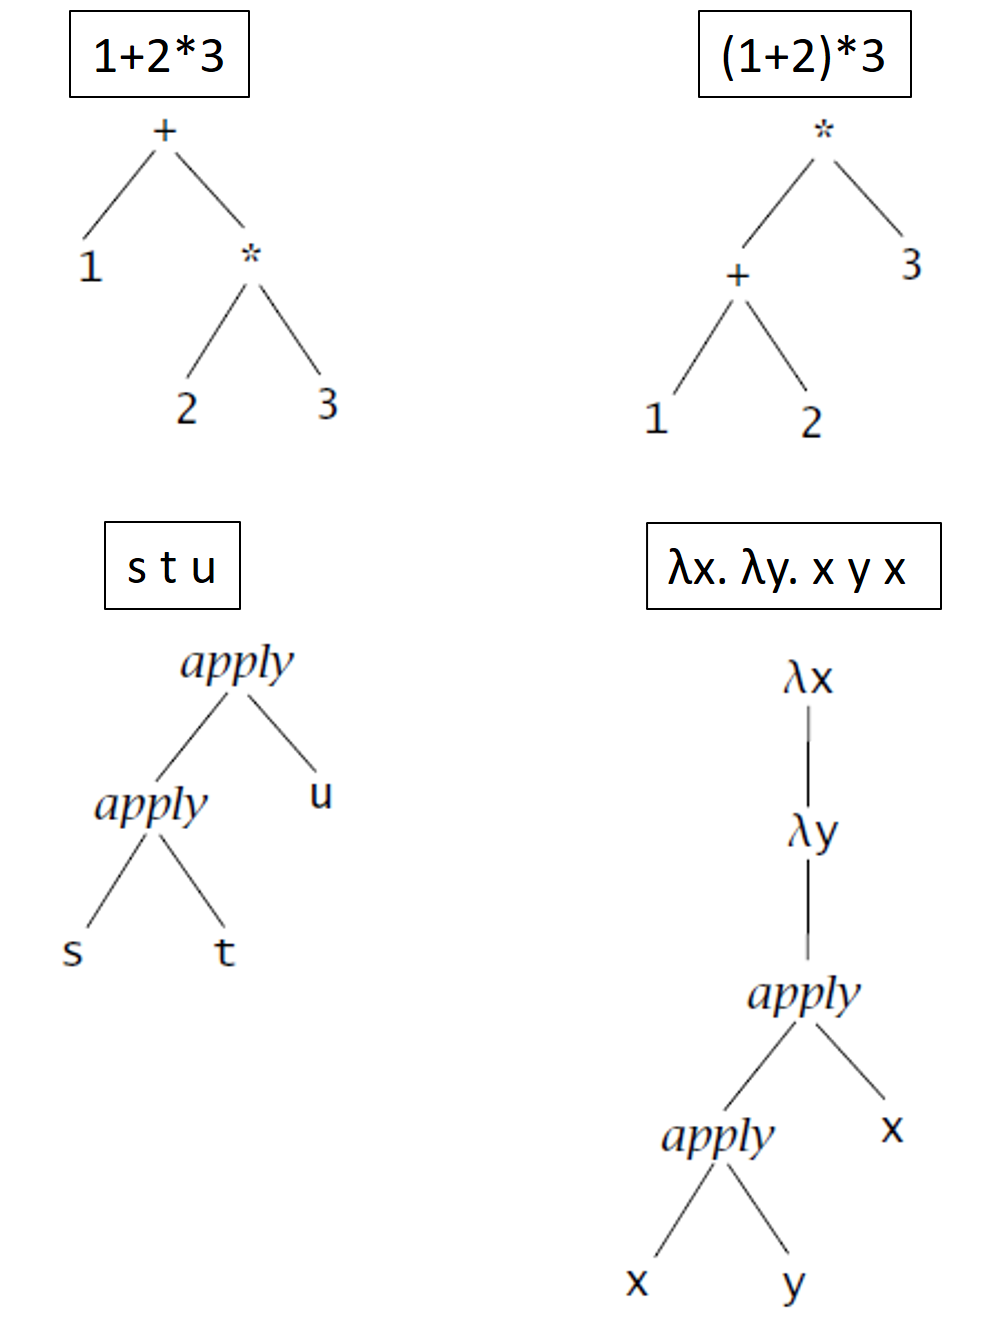
\includegraphics[width=5.5cm]{abstract_syntax_ch5}
\end{center}

\end{frame}

%%%
\begin{frame}[t]{5.1 Basics: variables vs. meta variables} 

The metavariables t (as well as s and u) to stand for an arbitrary term while the lambda calculus variable x (as well as y and z) to stand for an arbitrary variable. 

\vspace{10pt}

In a sentence like ``the term $\lambda$x. $\lambda$y. x y has the form $\lambda$z.s where \\ z = x and s = $\lambda$y. x y,''
\begin{itemize}
\item z and s are metavariables, whereas 
\item x and y are (lambda calculus) variables. 
\end{itemize}

\end{frame}


%%%
\begin{frame}[t]{5.1 Basics: scope}
The variable x is \underline{\it bound} when it occurs in the body of t of an abstraction $\lambda$x.t. Otherwise it is \underline{\it free}. 

\begin{itemize}
\item x is bound in $\lambda$x. {\color{red}x}
\item x is bound in $\lambda$z. $\lambda$x. $\lambda$y.  {\color{red}x} (y z) 
\item x is free in  {\color{red}x} y
\item x is free in $\lambda$y.  {\color{red}x} y
\item the first occurrence of x is bound and the second is free \\ in ($\lambda$x.  {\color{red}x})  {\color{red}x}
\end{itemize}

\vspace{10pt}

cf. $\lambda x$ is called a {\it binder}.

\vspace{10pt}

A term with no free variables is said to be \underline{\it closed}. Closed terms are called \underline{\it combinators}. 
\begin{itemize}
\item For example, ``$\lambda$x. x''  is an (identity) combinator.
\end{itemize}

\end{frame}

%%%
\begin{frame}[t]{5.1 Basics: operational semantics}

Substitution [x $\mapsto$ u] t: to replace all occurrences of x in t by u

\vspace{10pt}

A single step evaluation ($\rightarrow$) : \ \ 
\fbox{
($\lambda$x. t) u \ \ \ $\rightarrow$ \ \ \ [x $\mapsto$ u]t
}

\ \ cf. It is also called a reduction (or $\beta$-reduction). 

\vspace{10pt}

\begin{itemize}
\item ($\lambda$x. x) y  \ \ \ $\rightarrow$ \ \ \ y
\item ($\lambda$x. x ($\lambda$x. x)) \ (u r) \ \ \ $\rightarrow$ \ \ \  u r ($\lambda$x. x)
\end{itemize}

\vspace{10pt}

Several different evaluation strategies for the lambda calculus
\begin{itemize}
\item full beta-reduction, normal order reduction, 
\item call-by-name, \underline{\it call-by-value}
\end{itemize}

\end{frame}


%%%
\begin{frame}[t]{5.2 Programming in the Lambda-Calculus}

A warm-up exercises to get familiar with the lambda calculus by developing a number of standard examples of programming

\begin{itemize}
\item Multiple arguments
\item Church booleans
\item Pairs
\item Church numerals
\item Enriching the calculus
\item Recursion
\end{itemize}

\end{frame}


%%%
\begin{frame}[t]{5.2 Programming $\lambda$-calculus: Multiple Arguments} 

Multi-argument functions in a programming language, \\
 \ \ \ ``add = $\lambda$(x,y). x+y''

\vspace{10pt}

In the lambda calculus,  add = $\lambda$x. $\lambda$y. x+y 

\vspace{3pt}

\begin{tabular}{l l}
    & add 1 2 \\
 =  & (add 1) 2 \\    
 =  & (($\lambda$x. $\lambda$y. x+y) 1) 2 \\
 $\rightarrow$ & ($\lambda$y. 1+y) 2 \\
 $\rightarrow$ & 1+2  \\ 
 = & 3
\end{tabular}

\vspace{10pt}

\underline{\it Higher-order functions}: a function that takes or returns another function (e.g., add)

\vspace{10pt}

This transformation of multi-argument functions into higher-order functions is called {\it currying} in honor of Haskell B. Curry.

\end{frame}

%%%
\begin{frame}[t]{5.2 Programming $\lambda$-calculus: Church Booleans} 

Encoding boolean values and conditionals 

\vspace{10pt}

The terms tru and fls can be viewed as {\it representing} the boolean values ``true'' and ``false''.
\begin{itemize}
\item tru = $\lambda$t. $\lambda$f. t
\item fls = $\lambda$t. $\lambda$f. f 
\end{itemize}

\vspace{5pt}

We can define test as:
\begin{itemize}
\item test = $\lambda$l. $\lambda$m. $\lambda$n. l m n \ \ \ \ with the property that 
\begin{itemize} 
\item[(1)] (test b v w) reduces to v when b is tru, and 
\item[(2)] it reduces to w when b is fls. 
\end{itemize}
\end{itemize}

\vspace{10pt}

Q. Verify if test tru v w $\rightarrow \cdots \rightarrow$ v.

\vspace{5pt}

Q. Verify if test fls v w $\rightarrow \cdots \rightarrow$ w.

\end{frame}

%%%
\begin{frame}[t]{5.2 Programming $\lambda$-calculus: Church Booleans (Cont.)} \vspace{10pt}

We can also define boolean operators like logical conjunction as functions: 
\begin{itemize}
\item and = $\lambda$b. $\lambda$c. b c fls
\end{itemize}

\vspace{10pt}

Q. Verify if (and tru tru) becomes tru and the others (and tru fls, and fls tru, and fls fls) become fls).

\vspace{10pt}

Q. Define logical or and not functions.

\end{frame}

%%%
\begin{frame}[t]{5.2 Programming $\lambda$-calculus: Pairs} 

Making pairs, and selecting the first/the second member of a pair. 
\begin{itemize}
\item pair v w
\item (pair (pair a b) c)
\item (pair (pair a b) (pair c d))
\item fst (pair v w) becomes v.
\item snd (pair v w) becomes w.
\end{itemize}

\vspace{10pt}

The functions pair, fst, and snd:
\begin{itemize}
\item pair = $\lambda$f. $\lambda$s. $\lambda$b. b f s
\item fst = $\lambda$p. p tru
\item snd = $\lambda$p. p fls
\end{itemize}

\vspace{10pt}

Q. Show the last two properties on fst (pair v w) and snd (pair v w). 

\end{frame}

%%%
\begin{frame}[t]{5.2 Programming $\lambda$-calculus: Church numerals} 

Each number $n$ is represented by a function $c_n$ that takes two arguments, s and z, and applies s, n times, to z. 
\begin{itemize}
\item $c_0$ = $\lambda$s. $\lambda$z. z
\item $c_1$ = $\lambda$s. $\lambda$z. s z
\item $c_2$ = $\lambda$s. $\lambda$z. s (s z)
\item $c_3$ = $\lambda$s. $\lambda$z. s (s (s z))
\item $\cdots$
\item $c_n$ = $\lambda$s. $\lambda$z. s$^n$ z
\end{itemize}

\vspace{10pt}

Let us define addone to add 1 to an arbitrary number as
\begin{itemize}
\item addone = $\lambda$n. $\lambda$s. $\lambda$z. s (n s z)

\item For example, addone $c_1$ \\
$\rightarrow$ $\lambda$s. $\lambda$z. s ($c_1$ s z) \\
$\rightarrow$ $\lambda$s. $\lambda$z. s (($\lambda$z. s z) z) \\
$\rightarrow$ $\lambda$s. $\lambda$z. s (s z)
= $c_2$
\end{itemize}

\end{frame}

%%%
\begin{frame}[t]{5.2 Programming $\lambda$-calculus: Church numerals (Cont.)} 

The addition and multiplication of Church numerals by terms plus and times
\begin{itemize}
\item plus = $\lambda$m. $\lambda$n. $\lambda$s. $\lambda$z. m s (n s z)
\item times = $\lambda$m. $\lambda$n. m (plus n) $c_0$
\end{itemize}

\vspace{10pt}

Q. Try to reduce the following terms:
\begin{itemize}
\item plus $c_2$ $c_1$
\item times $c_2$ $c_1$
\end{itemize}

\end{frame}

%%%
\begin{frame}[t]{5.2 Programming $\lambda$-calculus: Church numerals (Cont.)} 

To test whether a Church numeral is zero, let us define a term iszro:
\begin{itemize}
\item iszro = $\lambda$m. m ($\lambda$x. fls) tru
\end{itemize}

\vspace{10pt}

Q. Compute the following terms using iszro:
\begin{itemize}
\item iszro $c_1$
\item iszro (times $c_0$ $c_2$)
\end{itemize}

\end{frame}

%%%
\begin{frame}[t]{5.2 Programming $\lambda$-calculus: Enriching the Calculus} \vspace{10pt}

Although we have seen that booleans, numbers, and the operations on them can be encoded in the pure lambda-calculus, it is often convenient to include the primitive booleans and numbers. 

\vspace{10pt}

The symbol $\lambda$ to refer to the pure lambda-calculus

\vspace{10pt}

The symbol $\lambda NB$ for the enriched system with booleans and arithmetic expressions from Ch.3

\end{frame}


%%%
\begin{frame}[t]{5.2 Programming $\lambda$-calculus: Recursion} \vspace{10pt}

The {\it divergent} combinator  \ \ \ \ \ cf. Combinators $\equiv$ closed terms 
\begin{itemize}
\item omega = ($\lambda$x. x x) ($\lambda$x. x x)
\item It only reduces to itself.
\end{itemize}

\vspace{10pt}

The omega combinator has a useful generalization called the \underline{\it fixed-point combinator}\footnote{Also called as (call-by-value) Y-combinator. A simpler version is fix = $\lambda$f. f (fix f), called as (call-by-name) Y-combinator.}
\begin{itemize}
\item fix = $\lambda$f. ($\lambda$x. f ($\lambda$y. x x y)) ($\lambda$x. f ($\lambda$y. x x y))
\end{itemize}

\vspace{10pt}

Use fix to define a recursive function, \\
 \ \ \ factorial = $\lambda$n. if n=0 then 1 else n * factorial (n-1):

\end{frame}

%%%
\begin{frame}[t]{5.2 Programming $\lambda$-calculus: Recursion (Cont.)} 
%\underline{\it Fixed-point combinator}
%\begin{itemize}
%\item fix = $\lambda$f. ($\lambda$x. f ($\lambda$y. x x y)) ($\lambda$x. f ($\lambda$y. x x y))
%\item (A simpler version is fix = $\lambda$f. f (fix f), called as Y-combinator.)
%\end{itemize}

\vspace{10pt}

To define a recursive function, \\
 \ \ \ factorial = $\lambda$n. if n=0 then 1 else n * {\color{red}factorial} (n-1):

\vspace{10pt}
 
First, make it {\it non-recursive} by replacing the recursive occurrence of factorial by an extra parameter fct as:

\vspace{5pt}

 \ \ \ nonrec\_factorial = {\color{red} $\lambda$fct.} $\lambda$n. if n=0 then 1 else n * {\color{red}fct} (n-1)

\vspace{10pt}

Then, apply fix to the non-recursive version to obtain the recursive behavior

\vspace{5pt}

 \ \ \ factorial = fix nonrec\_factorial

\vspace{20pt}

Q. Compute (factorial $c_3$). 

\end{frame}

%%%
\begin{frame}[t]{5.3 Formalities: the syntax \& operational semantics of $\lambda$-calculus}  \vspace{5pt}

Syntax: \\[0.1cm]

\begin{tabular}{l c l l } 
Term \texttt{t} & $::=$ &
	\texttt{x} & variable \\
	& $|$ & \texttt{$\lambda$x.t} & abstraction \\
	& $|$ & \texttt{t t} & application \\
Value \  \texttt{v} & $::=$ & \texttt{$\lambda$x.t} 
\end{tabular}

\vspace{10pt}

Evaluation: \\[0.1cm]

\begin{tabular}{c l} 
\mbox{
\begin{prooftree}
\hypo{ \texttt{t1} \rightarrow \texttt{t1'}  }
\infer1[]{ \texttt{t1 t2} \rightarrow \texttt{t1' t2} }
\end{prooftree}
}
&
(E-App1) \\[0.3cm]
\mbox{
\begin{prooftree}
\hypo{ \texttt{t2} \rightarrow \texttt{t2'}  }
\infer1[]{ \texttt{v1 t2} \rightarrow \texttt{v1 t2'} }
\end{prooftree}
}
&
(E-App2) \\[0.3cm]
\texttt{($\lambda$x. t) v} $\rightarrow$ \texttt{[x $\mapsto$ v] t} & (E-AppAbs)\\[0.3cm]
\end{tabular}

\end{frame}

%%%
\begin{frame}[t]{5.3 Formalities: Free variables, FV} \vspace{10pt}

FV(t) : the set of {\it free variables} of a term t
\begin{eqnarray*}
\texttt{FV(x)} &=& \texttt{\{ x \}} \\
\texttt{FV($\lambda$x. t1)} &=& \texttt{FV(t1) \textbackslash{} \{ x \}} \\
\texttt{FV(t1 t2)} &=& \texttt{FV(t1) $\cup$ FV(t2)} \\
\end{eqnarray*}

\vspace{10pt}

Q. Show the process of FV($\lambda$z. $\lambda$x. $\lambda$y.  x (y z) ).

\vspace{10pt}

Q. Define the size function for the lambda terms. 

\vspace{10pt}

Q. Show $|FV(t)| \leq size(t)$. 

\end{frame}


%%%
\begin{frame}[t]{5.3 Formalities: Substitution} \vspace{10pt}

The substitution operation [x $\mapsto$ s] t:

\begin{tabular}{l l l l}
\ [x $\mapsto$ s] x &=& s \\
\ [x $\mapsto$ s] y &=& y & if y $\not=$ x \\
\ [x $\mapsto$ s] ($\lambda$y. t1) &=& $\lambda$y. [x $\mapsto$ s]t1 & if y $\not=$ x and {\color{red}y $\not\in$ FV(s)} \\
\ [x $\mapsto$ s] (t1 t2) &=& \multicolumn{2}{l}{([x $\mapsto$ s] t1) ([x $\mapsto$ s] t2)} \\
\end{tabular}

\vspace{10pt}

Examples:
\begin{itemize}
\item \ 
[x $\mapsto$ ($\lambda$z. z w)] ($\lambda$y. x) = $\lambda$y. $\lambda$z. z w
\item \
[x $\mapsto$ y] ($\lambda$x. x) $\not=$ $\lambda$x. y  (It should be $\lambda$x. x)
\item \ 
[x $\mapsto$ z] ($\lambda$z. x) $\not=$ $\lambda$z. z  (It should be $\lambda$w. z after renaming z into w)
\end{itemize}

\vspace{10pt}

Alpha-conversion: renaming bound variables into new named ones

For example, [x $\mapsto$ y z]($\lambda${\color{red}y}. x {\color{red}y}) is renamed as [x $\mapsto$ y z]($\lambda${\color{red}w}. x {\color{red}w})
\end{frame}



\end{document}

